\def\year{2019}\relax
%File: formatting-instruction.tex
\documentclass[letterpaper]{article} %DO NOT CHANGE THIS
\usepackage{aaai19}  %Required
\usepackage{times}  %Required
\usepackage{helvet}  %Required
\usepackage{courier}  %Required
\usepackage{url}  %Required
\usepackage{graphicx}  %Required


%%%%%%%%%%%%% ADD CUSTOM PACKAGES TO macros.sty
\usepackage{macros}


\frenchspacing  %Required
\setlength{\pdfpagewidth}{8.5in}  %Required
\setlength{\pdfpageheight}{11in}  %Required
%PDF Info Is Required:
  \pdfinfo{
/Title (2019 Formatting Instructions for Authors Using LaTeX)
/Author (AAAI Press Staff)}
\setcounter{secnumdepth}{2}  
 \begin{document}
% The file aaai.sty is the style file for AAAI Press 
% proceedings, working notes, and technical reports.
%
\title{Submodular Bandits for Online Personalized Ranking}
\author{Author names withheld}
%\author{AAAI Press\\
%Association for the Advancement of Artificial Intelligence\\
%2275 East Bayshore Road, Suite 160\\
%Palo Alto, California 94303\\
%}
\maketitle
\begin{abstract}
To be written
\end{abstract}


\section{Introduction}
\label{intro}
In this paper, we study the problem of recommending the best items to users who are coming sequentially. The learner has access to very less prior information about the users (cold start) and it has to adapt quickly to the user preferences and suggest the best item to each user. We assume that the user-item preferences depends on latent factors. The learner only has access to noisy observations from the user-item preference matrix and the latent user or item features are not accessible. We further assume that the user-item preference matrix has low-rank, which is a very common assumption in recommender systems \citep{koren2009matrix}, \citep{ricci2011liorrokach}. %Also, we assume that each user has a single highest item.

	This complex problem can be conceptualized as a low rank online learning  problem where there are $K$ users and $L$ items. The user-item preference  matrix, denoted by $M\in [0,1]^{K\times L}$,  generating the feedback for user, item interaction has a low rank structure. The online learning game proceeds as follows, at every timestep $t$,  nature reveals one user (or row) \todoan{nature doesn't reveal the row, you can say row index} from $M$ where user is denoted by $i_t$. The learner selects $d$ items (or columns) from $[L]$, where an item is denoted by $j_t\in [L]$. Then the learner receives feedback $r_{t}(i_t,j_t)$ for all the $d$ items suggested from a noisy realization of $M$. This noisy realization of $M$ at time $t$ is denoted by $\tilde{M}_t(i_t,j_t)$ and  $r_{t}(i_t,j_t)] \sim \tilde{M}_t(i_t,j_t)$. Then the goal of the learner is to minimize the cumulative regret, that is to minimize the total number of wrong items displayed over time to the user. Hence, the learner needs to quickly identify the best item $j^*$ for each $i\in [K]$ where $M(i,j^*) = \argmax _{j\in[L]} M(i,j)$. \todoan{This doesn't completely explain our model where the permutation matters}
	
	This learning model is motivated from the real-world scenario where the learner has  to suggest movies to users and each movie belongs to a different genre (say thriller, romance, comedy, etc). So, the learner can suggest $d$ movies belonging to different genres to each incoming user on a webpage, and the user can click one, or all, or none of the recommended movies (query abandonement). \todoan{You can probably remove query abandonment comment.}	
	

	
% where $Ber$ is a Binomial distribution over the entries in $M$


\subsection{Related Works}
\label{related}
Our work lies at the intersection of several existing areas of research, which we survey below. 
\todoan{This can be compressed a lot. For one, if a there are just 1-2 papers using something, that shouldn't be part of a classification. This is the case, for example, when you say literature for latent bandits can be classified. You are describing things in too much detail. You can just say the setting which the other papers deal and why they they are different than this paper etc}

\textbf{Bandits for Latent Mixtures:} The existing algorithms in latent bandit literature can be broadly classified into two groups: the online matrix completion algorithms and the independent user model algorithms. The \textit{online matrix completion algorithms} try to reconstruct the user-item preference matrix $M$ from a noisy realization combining different approaches of online learning algorithms and matrix factorization algorithms. 
The NMF-Bandit algorithm in \citet{sen2016contextual} is an online matrix completion algorithm which is an $\epsilon$-greedy algorithm that tries to reconstruct the matrix $M$ through non-negative matrix factorization. Note, that this approach requires that all the matrices satisfy a weak statistical Restricted Isometric Property, which is not always feasible in real life applications. Another approach is that of \citet{gopalan2016low} where the authors come up with an algorithm which uses the Robust Tensor Power (RTP) method of 
\citet{anandkumar2014tensor} to reconstruct the matrix $M$, and then use the OFUL procedure of \citet{abbasi2011improved} to behave greedily over the reconstructed matrix. 
But the RTP is a costly operation because the learner needs to construct a matrix of order $L\times L$ and $L\times L \times L$ to calculate the second and third order tensors for the reconstruction.  A more simpler setting has also been studied in \citet{maillard2014latent} where all the users tend to come from only one class and hence this approach is also not quite realistic. 

The second type of algorithms are the \textit{independent user model algorithms} where for each user $i\in[K]$ a separate instance of a base-bandit algorithm is implemented to find the best item for the user. These base -bandits run independent of each other without sharing any information. These can be randomized algorithms suited for the adversarial setting like EXP3 \citep{auer2002nonstochastic} or UCB type algorithms suited for the stochastic setting llike UCB1 \citep{auer2002finite}, MOSS \citep{audibert2009minimax}, OCUCB \citep{lattimore2015optimally}, KL-UCB \citep{cappe2013kullback}, \citep{garivier2011kl} or even Bayesian algorithms like Thompson Sampling \citep{thompson1933likelihood}, \citep{thompson1935theory}, \citep{agrawal2012analysis}.

%can be used for this purpose.
%which are a set of frequentist indexed based algorithms
% Several powerful variation of the stochastic or non-stochastic multi-armed bandit algorithms can be used for this purpose.
%method with $\epsilon$ probability or with $1-\epsilon$ it behaves greedily over the already reconstructed matrix $\hat{M}$.

\textbf{Ranked Bandits:} Bandits have been used to rank items for online recommendations where the goal is is to present a list of $d$ items out of $L$ that maximizes the satisfaction of the user. A popular approach is to model each of the $d$ rank positions as a Multi Armed Bandit (MAB) problem and use a base-bandit algorithm to solve it. This was first proposed in \citet{radlinski2008learning} which  showed that query abandonment by user can also be successfully used to learn rankings. Later works on ranking such as \citet{slivkins2010ranked} and \citet{slivkins2013ranked} uses additional assumptions to handle  exponentially large number of items such that items and user models lie within a metric space and satisfy Lipschitz condition. 

\textbf{Ranking in Click Models:} Several algorithms have been proposed to solve the ranking problem in specific click models. Popular click models that have been studied extensively are Document Click Model (DCM), Position Based Click Model (PBM) and Cascade Click Model (CBM). For a survey of existing click models a reader may look into \citet{chuklin2015click}. While \citet{katariya2017bernoulli}, \citet{katariya2016stochastic} works in PBM, \citet{zoghi2017online} works in both PBM and CBM. Finally, \citet{kveton2017stochastic} can be viewed as a generalization of rank-1 bandits of \citet{katariya2016stochastic} to a higher rank. Note, that the theoretical guarantees of these algorithms does not hold beyond the specific click models.


\textbf{Online Sub-modular maximization:} Maximization of submodular functions has wide applications in machine learning, artificial
intelligence and in recommender systems \citep{nemhauser1978analysis}, \citep{krause2014submodular}. A submodular function $f : 2^V \rightarrow \mathbb{R}$ for a finite ground set $V$ is a set function that assign each
subset $S \subseteq V$ a value $f(S)$. We define the gain of the function $f$ as $G_f(e|S) = f(S \cup \lbrace e\rbrace) - f(S)$ where the element $\lbrace e\rbrace \in V\setminus S$ and $S \subseteq V$. Also, $f$ satisfies the following two criteria:-
\begin{enumerate}
\item Monotonicity: A set function $f : 2^V \rightarrow \mathbb{R}$ is monotone if for every $A \subseteq B \subseteq V, f(A) \leq f(B)$.
\item Submodularity: A set function $f : 2^V \rightarrow \mathbb{R}$ is submodular if for every $A \subseteq B \subseteq V$ and $\lbrace e\rbrace \in V \setminus B$ it holds that $G_f(e | A) \geq G_f(e | B)$.
\end{enumerate}

Intuitively, a submodular function states that after performing a set $A$ of actions, the marginal gain of another action $e$ does not increase the gain for performing other actions in $B \setminus A$. Online submodular function maximization has been studied in \citet{streeter2009online} where the authors propose a general algorithm whereas  \citet{radlinski2008learning} can be considered as special case of it when the payoff is only between $\lbrace 0, 1\rbrace$. Also, in the contextual feature based setup online  submodular maximization has been studied by  \citet{yue2011linear}. An interesting property of submodular function is that a greedy algorithm using it is guaranteed to perform atleast $\left( 1 - \frac{1}{e}\right)$ of the optimal algorithm and this factor $\left( 1 - \frac{1}{e}\right)$ is not improvable by any polynomial time algorithm \citep{nemhauser1978analysis}.




\subsection{Notations, Problem Formulation and Assumptions}
We define $[n] = \lbrace 1,2,\ldots, n\rbrace$ and for any two sets $A$ and $B$, $A^B$ denotes the set of all vectors who take values from $A$ and are indexed by $B$. Let, $M\in [0,1]^{K\times L}$ denote any matrix, then $M(I,:)$ denote any submatrix of $k$ rows such that $I\in[K]^k$ and similarly $M(:,J)$ denote any submatrix of $j$ columns such that $J\in[L]^{j}$.
	
	Let $M$ be reward matrix of  dimension $K\times L$ where $K$ is the number of user or rows and $L$ is the number of arms or columns. Also, let us assume that this matrix  $M$ has a low rank structure of rank $d << \min\lbrace L,K\rbrace$. Let $U$ and $V$ denote the latent matrices for the users and items, which are not visible to the learner such that,
\begin{align*}
	M = UV^{\intercal} \textbf{ \hspace*{4mm}   s.t.   \hspace*{4mm}} U\in [ \mathbb{R}^+ ]^{K\times d} \textbf{, } V\in  [0,1]^{L\times d} 
\end{align*}	  
	
	Furthermore, we put a constraint on $V$ such that, $\forall j\in [L]$, $ \norm{V(j,:)}_1 \leq 1$. 
	
	
\begin{assumption}\textbf{(Hott-Topics)}
\label{assm:1}
We assume that there exists $d$-column base factors, denoted by $V(J^*,:)$, such that all rows of $V$ can be written as a convex combination of $V(J^*,:)$ and the zero vector and $J^* = [d]$. We denote the column factors by $V^* = V(J*,:)$. Therefore, for any $i\in [L]$, it can be represented by
\begin{align*}
V(i,:) = a_i V(J^*,:) , 
\end{align*}
where $\exists a_i\in [0,1]^{d}$ and $ \norm{a_i}_1 \leq 1$.
\end{assumption}

%In this paper, in addition to the noisy setting explained in section \ref{intro} we first analyze the proposed algorithm in the easier noise free setting. In the noise free setting, the nature reveals the row $i_t$, and when the learner selects the column $j_t$, it observes the mean of the distribution $\bar{R}(i_t,j_t)$.

%\begin{assumption}
%\label{assm:round-robin}
%We assume that nature is revealing the user $i$ in $\bar{R}(i,:), \forall i\in [K]$  in a Round-Robin fashion such that at timestep $t$, nature reveals $i_t = (t \mod K) + 1$.
%\end{assumption}

\begin{assumption}\textbf{(Click Model)}
\label{assm:d-items}
For each user $i_t$ revealed by the nature at round $t$, the learner is allowed to suggest atmost $d$-items, where $d$ is the rank of the matrix $\bar{R}$. The user can click one, or all, or none of the recommendations.
\end{assumption}

\begin{discussion}
The above Assumption \ref{assm:d-items} can be conceptualized in this real-world scenario where the learner has  to suggest movies to users and each movie belongs to a different genre (say thriller, romance, comedy, etc). So, the learner can suggest $d$ movies belonging to different genres to each user in a webpage, and the user can click one, or all, or none of the recommended movies (query abandonement).
\end{discussion}

The main goal of the learning agent is to minimize the cumulative regret until the end of horizon $n$. We define the cumulative regret, denoted by $\mathcal{R}_n$ as,

\begin{align*}
\mathcal{R}_n = \sum_{t=1}^{n}\bigg\lbrace \sum_{z=1}^{d} \bigg( r_{t}\left(i_{t}, j^* \right) - r_{t}\left( i_{t}, j_{t,z}\right)\bigg)\bigg\rbrace
\end{align*}

where, $j^* = \argmax_{j\in [L]}\lbrace M(i_t,j)\rbrace$ and $j_{t,z}$ be the suggestion of the learner for the $i_t$ -th user for  $z=1,2,\ldots, d$. Note that $r_{t}\left(i_t, j^* \right)\sim Ber(M\left(i_t, j^*\right))$ and $r_{t}\left(i_t, j_{t,z} \right)\sim Ber(M\left(i_t, j_{t,z} \right))$. Taking expectation over both sides, we can show that,

\begin{align*}
\E[\mathcal{R}_n] & = \E\left [ \sum_{t=1}^{n}\bigg\lbrace\sum_{z=1}^{d} \bigg( r_{z,t}\left(i_t, j^* \right) - r_{z, t}\left( i_t, j_{z, t}\right)\bigg)\bigg\rbrace\right] \\
%%%%%%%%%%%%%%%%%%%%
&= \E\left [ \sum_{t=1}^{T} \sum_{z=1}^{d} \bigg( N_{i_t,j_{z,t}}\bigg) \right ]\Delta_{i_t,j_{z,t}}
\end{align*}

where, $\Delta_{i_t,j_{z,t}} = M(i_t,j^*) - M(i_t,j_{z,t})$ and $N_{i_t,j_{z,t}}$ is the number of times the learner has observed the $j_{z,t}$-th item for the $i_t$-th user. Let, $\Delta = \min_{i\in[K],j\in[L]}\lbrace \Delta_{i,j}\rbrace$ be the minimum gap over all the user, item pair in $M$.



\section{Contributions}
Our contributions are mainly three fold. First, we formulate the latent ranked bandit problem as an online learning problem on a class of low-rank non-negative matrices that can be solved efficiently without estimating the latent factors that generate the matrices. We borrow ideas from the ranking literature to solve this problem efficiently and term this setting as personalized ranking setting. This is because an efficient algorithm can find a global ranking of best items and then permute that list to find a personalized ranking for individual users, sorted in descending order of their preference towards item. Secondly, we propose the latent ranker algorithm (LRA) for this personalized ranking setting. LRA has two components, the column algorithms that suggests $d$ columns and the row ranking component which permutes that suggested list to find the best permutation amongst them. The best permutation is personalized for each user such that it will contain the best item for that user at rank $1$ position with high probability. The column algorithms leverage the low rank structure of the user-preference matrix $M$ and quickly finds out the $d$ best items. Simultaneously the row ranking components observe all the feedback from the user permute the suggested list of $d$ items to find the highest reward permutation such that the best item is at rank $1$ position for the individual users. Finally, we show that an instance of LRA which uses exponential weighting algorithm EXP3 as column MABs and weighted majority algorithm (WMA) as row MABs suffer a regret of atmost $O\left(\frac{d \sqrt{L n}}{\Delta} + K \log n + K d \log d\right)$. On diverse experimental settings we test our proposed algorithm and show improved performance even when our modeling assumptions does not hold.

	The rest of the paper is organized as follows. We state our setting, assumptions and notations in Section \ref{sec:setting}. We propose the algorithm LRA in Section \ref{sec:algorithm} and in Section \ref{sec:analysis} we analyze LRA. Finally, we show experiments in Section \ref{sec:expt} and give a brief survey of the existing literature in Section \ref{sec:related}. We conclude in Section \ref{sec:conclusions} while the proof is contained in the Appendix \ref{sec:proof}.

\newpage
\section{Proposed Algorithms}
We propose the algorithm Latent Ranked Bandit, abbreviated as LRB (see Algorithm \ref{alg:latent-rank}) for solving the personalized ranking problem. This algorithm is motivated by the Ranked Bandit Algorithm (RBA) from \citet{radlinski2008learning} which is suited for finding a global ranking amongst all the users in the CBM click model. LRB is divided into two main components, the $d$ column MABs denoted by MAB$_1(n)$, MAB$_2(n), \dots,$ MAB$_d(n)$ and the $K$ row Weighted Majority Algorithms (WMA) for each user $[K]$. The WMA is motivated from \citet{littlestone1994weighted} which is suited for the total information setting. Note, that in our DCM setting all the clicks by the user is seen by the system and so it is a variation of total information setting. Each WMA consist of $d!$ arms for each of the permutations of rank $d$. Its main goal is to suggest a permutation $\Pi_{i_t}(S_t), \exists S_t \subseteq [L]$ such that the best item for the user $i_t$ is in rank $1$ of the permutation $\Pi_{i_t}(S_t)$.  LRB proceeds as follows, at every timestep $t\in[n]$ a user $i_t$ is revealed by nature, then the $d$ column MABs suggests columns $S_t = \lbrace {\ell}_{1}, {\ell}_{2},\dots, {\ell}_{d} \rbrace$ which it deems to be the $d$ best columns and by virtue of our setting, the $d$ hott-topics. If, there is any overlap in the suggestion, an arbitrary column is suggested which has not been selected before. Then, the row WMA for the $i_t$-th user selects a permutation $\Pi_{i_t}(S_t)$ by sampling through its distribution over the $d!$ arms and suggests a permutation $\tilde{S}_t = \lbrace \tilde{\ell}_{1}, \tilde{\ell}_{2},\dots, \tilde{\ell}_{d}\rbrace$ such that the item in rank $1$ is the best item for the $i_t$-th user with a high probability. Note, that we leave the implementation of the column MAB to the user which can be any stochastic or adversarial base-bandit algorithm discussed in Section \ref{related}.

Finally, after all the user clicks are recorded by the system both the column MABs and row WMA$_{i_t}(n)$ is updated. The $k$-th column bandit MAB$_k(n)$ is updated with feedback $f_{k,t} = \max_{j\in [k]} r_t(i_t, \ell_{j,t}) - \max_{j\in [k-1]} r_t(i_t,\ell_{j,t})$ such the monotonicity and submodularity properties discussed in section \ref{related} are maintained. Note that RBA is also a special case of submodular bandits such that $f_{k,t}\in\lbrace 0, 1\rbrace$ \citep{streeter2009online}. 


The row WMA$_{i_t}(n)$ update for the $i_t$-th user is quite straightforward as all the $d$ clicks are observed (total information). Hence, LRB can easily calculate the feedback for all the $d!$ permutation of $\Pi_{i_t}(S_t)$ and update its $d!$ arms representing each of those permutations. LRB calculates a weighted sum of feedback for each of the $d!$ permutation of $\Pi_{i_t}(S_t)$ and update the weights and its probabilities of the corresponding permutation. An illustrative diagram of the entire process is shown in Figure \ref{fig:rankedbandit}.

%Since, we observe all the clicks by user $i_t$ (total information),
\begin{figure}[!th]
    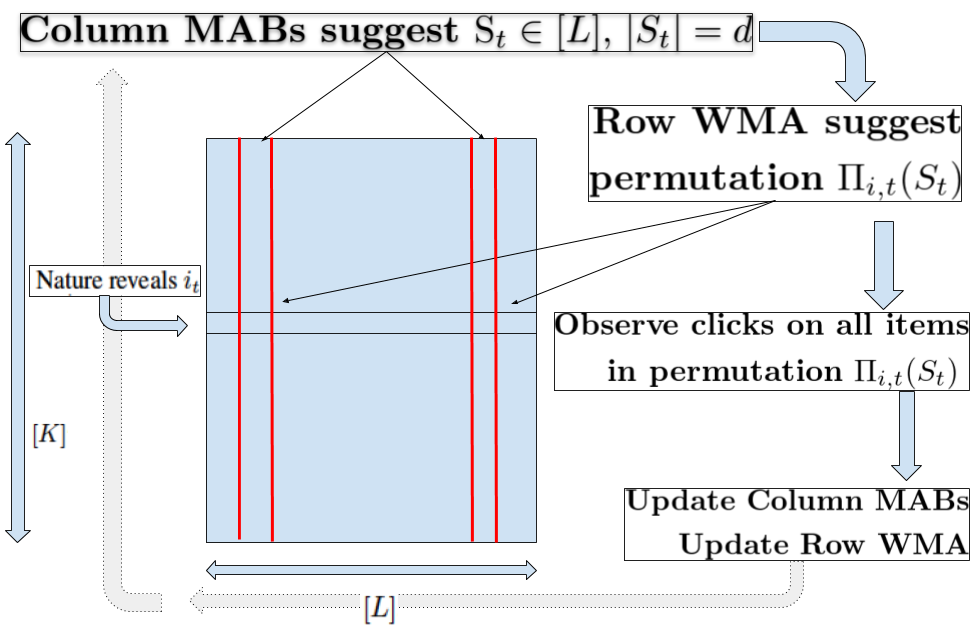
\includegraphics[scale=0.2]{img/RankedBand.png}
    \caption{Latent Ranked Bandit in rank $d=2$ scenario.}
    \label{fig:rankedbandit}
    \vspace*{-1em}
\end{figure}

\begin{algorithm}
\caption{Latent Ranked Bandit}
\label{alg:latent-rank}
  \begin{algorithmic}[1]
  \State \textbf{Input:} Rank $d$, horizon $n$.
  \State Initialize MAB$_1(n)$, MAB$_2(n), \dots,$ MAB$_d(n)$
  \State Initialize WMA$_1(n)$, WMA$_2(n), \dots,$ WMA$_K(n)$
    \For{$t = 1, \dots, n$}
      \State User $i_t$ comes to the system
      \For{$k = 1, \dots, d$}
      %\State // Choose $d$ items from $d$ column MABs
      \State ${\ell}_{k,t} \leftarrow$ suggest item $MAB_k(n)$
      \If{${\ell}_{k,t} \in \ell_{1, t},\dots,\ell_{k-1, t}$}
      \State ${\ell}_{k,t} \leftarrow$ Select arbitrary unselected item from $[L]\setminus \ell_{1, t},\dots,\ell_{k-1, t}$
      %\Else
      %\State $\ell_{k,t} \leftarrow \hat{\ell}_{k,t}$
      \EndIf
      \EndFor
      \State $\tilde{\ell}_{1,t},\tilde{\ell}_{2,t},\dots,\tilde{\ell}_{d,t}\leftarrow$ Permutation by WMA$_{i_t}(\ell_{1,t},\ell_{2,t},\dots,\ell_{d,t})$ by sampling  according to $p_{i_t,1},p_{i_t,2},\dots,p_{i_t,d!}$.
      %by sorting descendingly according to $w_{i_t,1},w_{i_t,2},\dots,w_{i_t,d}$.
      \State Present $\tilde{\ell}_{1,t},\tilde{\ell}_{2,t},\dots,\tilde{\ell}_{d,t}$ to user $i_t$ and record feedback $r_{t}(\tilde{\ell}_{1,t}), r_{t}(\tilde{\ell}_{2,t}),\dots,r_{t}(\tilde{\ell}_{d,t})$.
      \State Call Procedure UpdateColumnMAB
      \State Call Procedure UpdateRowWMA($i_t$)
    \EndFor
    \Procedure{UpdateColumnMAB}{}
    \For{$k = 1, \dots, d$}
    \State Update MAB$_k(n)$ with feedback $f_{k,t} = \max_{j\in [k]} r_t(i_t, \ell_{j,t}) - \max_{j\in [k-1]} r_t(i_t,\ell_{j,t})$
    % where $J_t[1: k] = \lbrace r_{t}({\ell}_{1,t}), r_{t}({\ell}_{2,t}),\dots,r_{t}({\ell}_{k,t})\rbrace$
    \EndFor
\EndProcedure
\Procedure{UpdateRowWMA}{$i_t$}
	\For{$k=1,2,\dots,d!$}
	\State $r_k = 0$ \Comment{Calculate weighted sum of rewards}
    \For{$j = 1, \dots, d$}
    \State $r_{k} = r_{k} + \frac{1}{j}r_{t}(\tilde{\ell}_{j,t})$
    \EndFor
    \State $w_{i_t,k} = w_{i_t,k} + r_k$  \Comment{Update weights}
    \EndFor
	\For{$k = 1, \dots, d!$}
	\State $p_{i_t,k} = \dfrac{\exp(w_{i_t,k})}{\sum_{b=1}^{d!} \exp(w_{i_t,b})} $ %\Comment{Update probabilities}
	\EndFor
\EndProcedure
  \end{algorithmic}
\end{algorithm}

\newpage
\section{Experiments}
In this section, we conduct three experiments and evaluate the performance of LRB against several bandit algorithms. Note, that at every timestep $t$, nature reveals an user $i_t$ and each algorithm suggests $d$ items to it and records all the $d$ feedbacks. The first two experiments are on simulated dataset where all our modelling assumptions hold. The third experiment is on a real-life dataset where we evaluate LRB when our modelling assumptions fail. In all our experiments users come in a Round Robin fashion over all time $[n]$. All the algorithms are averaged over $10$ independent runs.

\textbf{Contextual Algorithms:} In the contextual approach, each user has a separate version of base-bandit algorithm running independent of each other. As base-bandit algorithms we choose two versions of stochastic MAB, UCB1 and Thompson Sampling (TS), abbreviated as Contextual UCB1 (CUCB1) and Contextual TS (CTS) respectively. For UCB1, we choose the confidence interval at timestep $t$ as $c_{i_t, j}(t) = \sqrt{\frac{1.5 \log t}{N_{i_t,j}(t)}}$ for the $i_t$-th user and $j$-th item. Note, that both the vanilla UCB1 and TS is used to find the best item for each user at rank $1$, while for the remaining positions $k= 2,\dots, d$ it  suggest previously unselected items by sampling uniform randomly at every timestep $t$. 

\textbf{Matrix Completion Algorithms:} In the matrix completion approach, the algorithms try to reconstruct the user-item preference matrix $M$ from its noisy realization. We use two widely used method to reconstruct partially observed noisy matrices, linear ridge regression and non-negative matrix factorization. We term the corresponding algorithms as Linear Bandit (LinBan) and NMF Bandit (NMF-Ban) respectively. Both of these algorithms are $\epsilon$-greedy in implementation whereby they reconstruct $M$ with $\epsilon$ probability and with $1-\epsilon$ probability they behave greedily over the reconstructed matrix and suggest $d$ best item for the $i_t$-th user at every timestep $t$. LinBan uses ridge regression to reconstruct $M$ from its estimated $d$-best columns while NMF-Ban uses matrix factorization to estimate the $U$ and $V$ matrix and reconstruct $M$ from its noisy realization.

\textbf{Personalized Ranking Algorithms:} In this approach, we evaluate our proposed algorithm Latent Ranking Bandit (LRB) by using two different types of base-bandits, EXP3 and UCB1 as column MABs. We term them as LREXP3 and LRUCB1 respectively. For LREXP3 we set the column exploration parameter $\gamma_k = \sqrt{\frac{L \log L}{n}}, \forall \text{ MAB}_k(n), k = 1,\dots, d$ and for LRUCB1 we use  a confidence interval of $c_{k, j}(t) = \sqrt{\frac{1.5 \log t}{N_{k,j}(t)}}$ for the $k$-th column MAB and $j$-th item.

\textbf{Experiment 1:} This experiment is conducted to test the performance of LRB over  small number of users and items. This simulated testbed consist of $500$ users, $50$ items and rank$(M) = 2$. The vectors spanning $U$ and $V$, generating the user-item preference matrix $M$ is shown Figure \ref{fig:1}. The users are divided into a $70:30$ split such that $70\%$ of users prefer item $j^*_1$ and $30\%$ users prefer item  $j^*_2$. The hott-topics are $V(1:) = (0,1)$ and $V(2,:) = (1, 0)$ while remaining $70\%$ of items belong to $V(\ell_{j'},:) = (0.45, 0.55)$ and the rest to $V(\ell_{j}) = (0.55, 0.45)$. We create the user feature matrix $U$ similarly having a $70:30$ split. The resultant matrix $M =UV^{\intercal}$ is such that algorithms that quickly find the easily identifiable hott-topics perform very well. From Figure \ref{fig:2} we can clearly see that both LREXP3 and LRUCB1 outperforms all the other algorithms. Their regret curve flattens, indicating that they have learned the best items for each user.  NMF-Ban and LinBan has nearly similar performance as both of these algorithms fail to get a reasonable approximation of $M$ although they perform better than CUCB1. Contextual algorithm CUCB1 performs poorly as the number of items per user is too large and the gaps are also small. Although CTS performs well in this small testbed, its performance eventually degrades for larger environments. 


\begin{figure}[!th]
\centering
\begin{tabular}{cc}
\setlength{\tabcolsep}{0.1pt}
\subfigure[0.25\textwidth][Expt-$1$: $500$ Users, $50$ items, Rank $2$, User and Item vectors]
    %with $r_{i_{{i}\neq {*}}}=0.07$ and $r^{*}=0.1$
    {
    		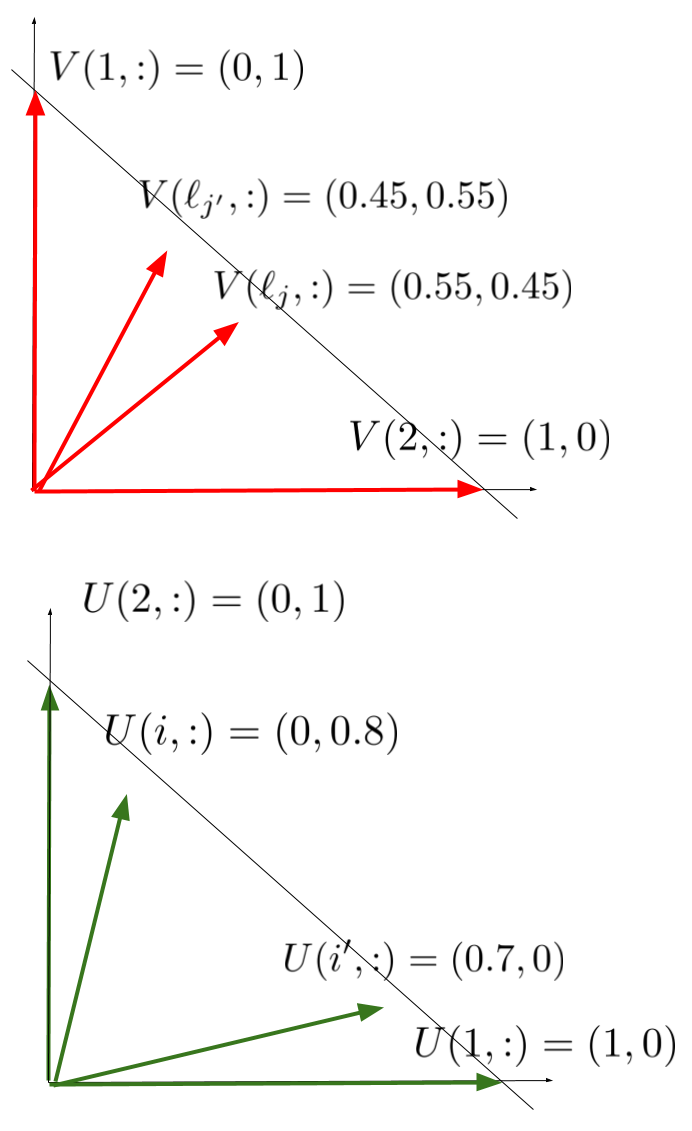
\includegraphics[scale=0.11]{img/rank2_vec.png}
  		\label{fig:1}
    }
    &
    \subfigure[0.25\textwidth][Expt-$1$: Cumulative regret of different algorithms]
    %with $r_{i_{{i}\neq {*}}}=0.07$ and $r^{*}=0.1$
    {
    		\pgfplotsset{
		tick label style={font=\Large},
		label style={font=\Large},
		legend style={font=\Large},
		ylabel style={yshift=5pt},
		%legend style={legendshift=32pt},
		}
        \begin{tikzpicture}[scale=0.4]
      	\begin{axis}[
		xlabel={timestep},
		ylabel={Cumulative Regret},
		grid=major,
        %clip mode=individual,grid,grid style={gray!30},
        clip=true,
        %clip mode=individual,grid,grid style={gray!30},
        cycle list name=exotic,
  		legend style={at={(0.5,1.4)},anchor=north, legend columns=3} ]
      	% UCB
		\addplot table{results/NewExpt1/Expt1/comp_subsampled_CTS0RR1S.txt};
		\addplot table{results/NewExpt1/Expt1/comp_subsampled_LRUCB0RR1S.txt};
		\addplot table{results/NewExpt1/Expt1/comp_subsampled_LREXP30RR1S.txt};
		\addplot table{results/NewExpt1/Expt1/comp_subsampled_NMF0RR1S.txt};
		\addplot table{results/NewExpt1/Expt1/comp_subsampled_LinBan0RR1S.txt};
		\addplot table{results/NewExpt1/Expt1/comp_subsampled_CUCB10RR1S.txt};
		\legend{CTS, LRUCB1, LREXP3, NMF-Ban, LinBan, CUCB1} 
      	\end{axis}
      	\end{tikzpicture}
  		\label{fig:2}
    }
    \\
    \subfigure[0.25\textwidth][Expt-$2$: $1500$ Users, $100$ items, Rank $3$, User and Item vectors]
    %with $r_{i_{{i}\neq {*}}}=0.07$ and $r^{*}=0.1$
    {
    		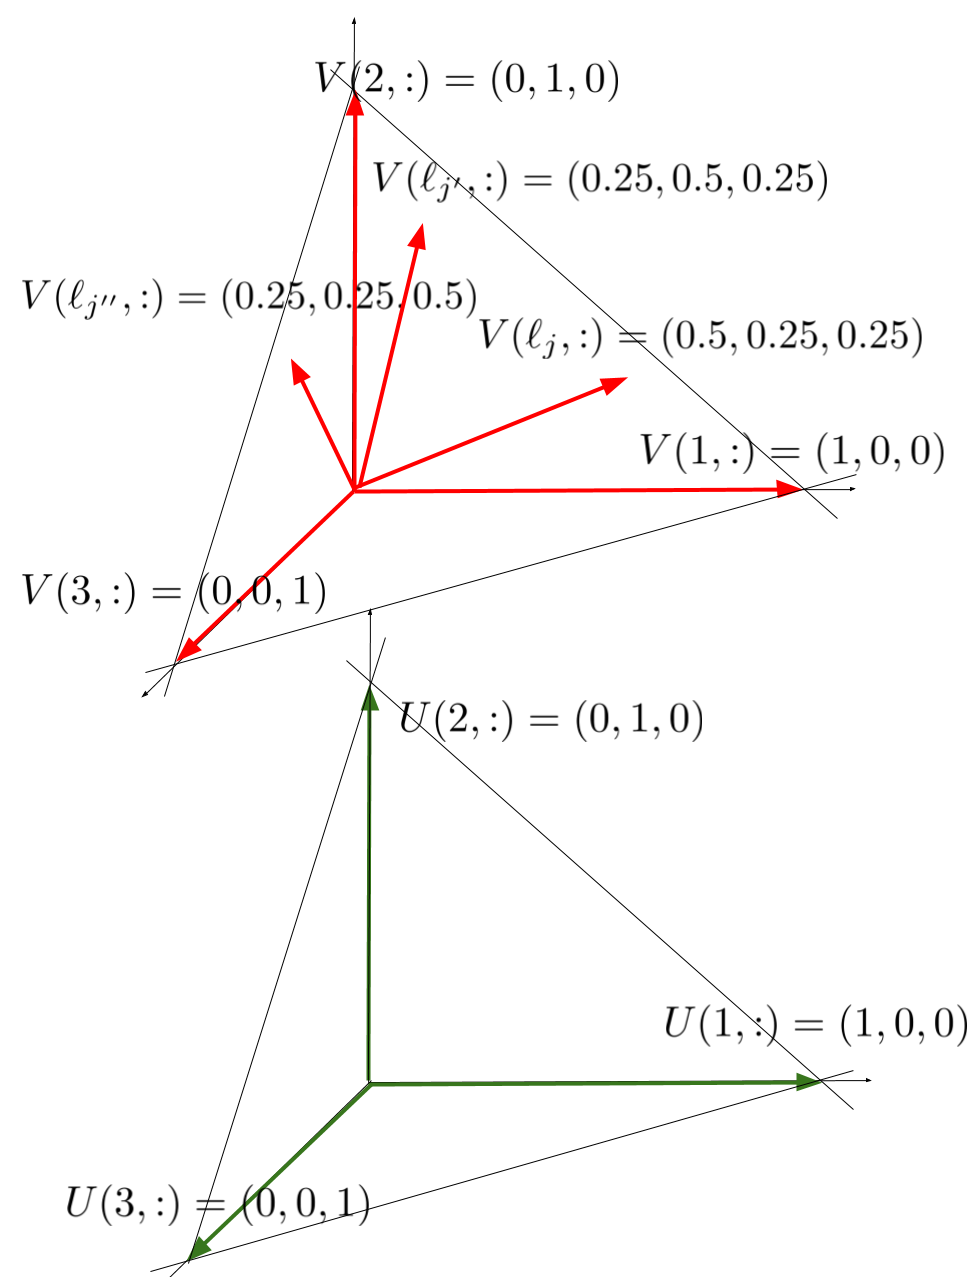
\includegraphics[scale=0.11]{img/rank3_vec.png}
  		\label{fig:3}
    }
    &
    \subfigure[0.25\textwidth][Expt-$2$: Cumulative regret of different algorithms]
    %with $r_{i_{{i}\neq {*}}}=0.07$ and $r^{*}=0.1$
    {
    		\pgfplotsset{
		tick label style={font=\Large},
		label style={font=\Large},
		legend style={font=\Large},
		ylabel style={yshift=5pt},
		%legend style={legendshift=32pt},
		}
        \begin{tikzpicture}[scale=0.4]
      	\begin{axis}[
		xlabel={timestep},
		ylabel={Cumulative Regret},
		grid=major,
        %clip mode=individual,grid,grid style={gray!30},
        clip=true,
        %clip mode=individual,grid,grid style={gray!30},
        cycle list name=exotic,
  		legend style={at={(0.5,1.4)},anchor=north, legend columns=3} ]
      	% UCB
		\addplot table{results/NewExpt1/Expt2/comp_subsampled_CTS0RR1S.txt};
		\addplot table{results/NewExpt1/Expt2/comp_subsampled_LRUCB0RR1S.txt};
		\addplot table{results/NewExpt1/Expt2/comp_subsampled_LREXP30RR1S.txt};
		\addplot table{results/NewExpt1/Expt2/comp_subsampled_NMF0RR1S.txt};
		\addplot table{results/NewExpt1/Expt2/comp_subsampled_LinBan0RR1S.txt};
		\addplot table{results/NewExpt1/Expt2/comp_subsampled_CUCB10RR1S.txt};
		\legend{CTS, LRUCB1, LREXP3, NMF-Ban, LinBan, CUCB1} 
      	\end{axis}
      	\end{tikzpicture}
  		\label{fig:4}
    }
    \end{tabular}
    \caption{A comparison of the cumulative regret incurred by the various bandit algorithms. }
    \label{fig:karmed1}
    \vspace*{-1em}
\end{figure}

\textbf{Experiment 2:} We conduct the second experiment on a larger simulated database of $1500$ users, $100$ items and rank$(M)=3$. The vectors spanning $U$ and $V$, generating the user-item preference matrix $M$ is shown Figure \ref{fig:3}. The users are divided into a $60:30:10$ split such that $60\%$ of the users prefer item $j^*_1$, $30\%$ prefer $j^*_2$ and $10\%$ prefer $j_3^*$.  Here, hott-topics are $V(1,:) = (1,0,0)$, $V(2,:) = (0,1, 0)$ and $V(3,:) = (0,0,1)$. The remaining $60\%$ of items belong to $V(\ell_{j},:) = (0.5, 0.25,0.25)$, $30\%$ to $V(\ell_{j'}) = (0.25, 0.5, 0.25)$ and rest to $V(\ell_{j''}) = (0.25, 0.25, 0.5)$. We create the user feature matrix $U$ similarly having a $60:30:10$ split and the vectors spanning $U$ are only of the type that spans the simplex, i.e $\lbrace 1,0,0\rbrace$, $\lbrace 0,1,0 \rbrace$ and $\lbrace 0,0,1 \rbrace$. Again, the resultant matrix $M =UV^{\intercal}$ is such that algorithms that quickly spot the easily identifiable hott-topics outperform others. From Figure \ref{fig:4} we can see that both LREXP3 and LRUCB1 again outperforms all the other algorithms. Their regret curve flattens much before all the other algorithms indicating that they have learned the best items for each user. The matrix completion algorithms NMF-Ban and LinBan fail to get a reasonable approximation of $M$ and perform poorly. Also, we see that both the contextual algorithms CUCB1 and CTS perform poorly as the number of users and the number of items per user is too large and the independent base-bandits are not sharing information between themselves. In both the simulated datasets, we see that stochastic column MAB (UCB1) is outperforming adversarial column MAB (EXP3) as the user preference over the best item is not changing over time. This has also been observed by \citet{radlinski2008learning}.

%which stems from the fact that all the user, 

\textbf{Experiment 3:} We conduct the third experiment to test the performance of LRB when our modelling assumptions are violated. We use the Jester dataset \citep{goldberg2001eigentaste} which consist of over 4.1 million continuous ratings of 100 jokes from 73,421 users collected over 5 years. We sample randomly around 2000 users from this dataset and use singular value decomposition (SVD) to obtain a rank $2$ approximation of this user-joke rating matrix $M$. The rank $2$ approximation of $M$ of  is shown in Figure \ref{fig:5}, where we can clearly see the red stripes spanning the matrix indicating the low-rank structure of $M$. Furthermore, in this experiment we assume that the noise is independent Bernoulli over the entries of $M$ and hence this experiment deviates from our modeling assumptions. From \ref{fig:6} again we see that LREXP3 outperforms other algorithms. The regret curve of LRUCB1 does not flatten out which we attribute to the fact that LRUCB1 uses too large a confidence interval. The contextual and matrix completion algorithms perform significantly worse in this large testbed.



%[[1104, 99], [896, 93],[0,0][0,0]}

\begin{figure}[!th]
\centering
\begin{tabular}{cc}
\setlength{\tabcolsep}{0.1pt}
\subfigure[0.25\textwidth][Expt-$3$: $2000$ Users, $100$ items, Rank $2$ approximation of Jester Dataset]
    %with $r_{i_{{i}\neq {*}}}=0.07$ and $r^{*}=0.1$
    {
    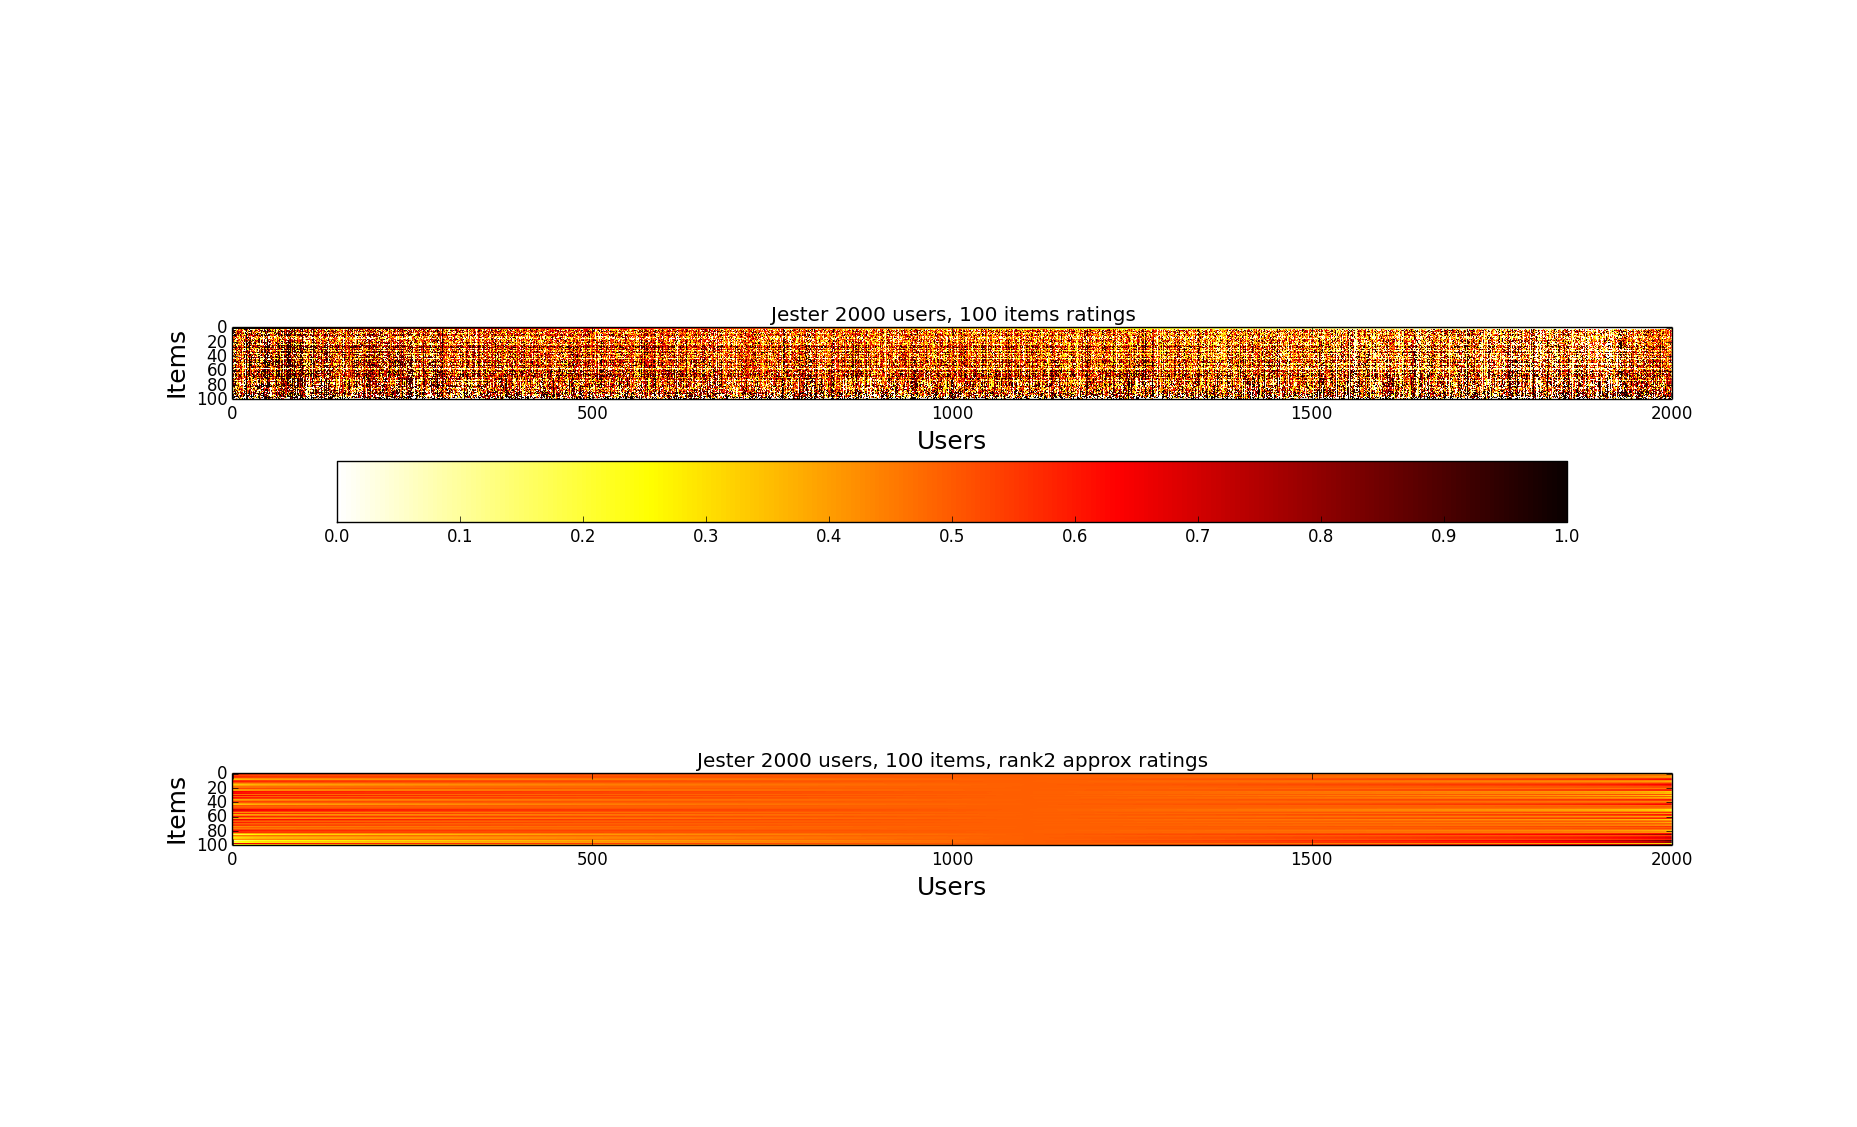
\includegraphics[scale=0.08]{img/jester_rank2.png}
    	\label{fig:5}
    }
    &
\subfigure[0.25\textwidth][Expt-$3$: Cumulative regret of different algorithms]
    %with $r_{i_{{i}\neq {*}}}=0.07$ and $r^{*}=0.1$
    {
    		\pgfplotsset{
		tick label style={font=\Large},
		label style={font=\Large},
		legend style={font=\Large},
		ylabel style={yshift=5pt},
		%legend style={legendshift=32pt},
		}
        \begin{tikzpicture}[scale=0.4]
      	\begin{axis}[
		xlabel={timestep},
		ylabel={Cumulative Regret},
		grid=major,
        %clip mode=individual,grid,grid style={gray!30},
        clip=true,
        cycle list name=exotic,
        %clip mode=individual,grid,grid style={gray!30},
  		legend style={at={(0.5,1.4)},anchor=north, legend columns=3} ]
      	% UCB
		
		\addplot table{results/NewExpt1/Expt3/comp_subsampled_CTS0RR1S.txt};
		\addplot table{results/NewExpt1/Expt3/comp_subsampled_LRUCB0RR1S.txt};
		\addplot table{results/NewExpt1/Expt3/comp_subsampled_LREXP30RR1S.txt};
		\addplot table{results/NewExpt1/Expt3/comp_subsampled_NMF0RR1S.txt};
		\addplot table{results/NewExpt1/Expt3/comp_subsampled_LinBan0RR1S.txt};
		\addplot table{results/NewExpt1/Expt3/comp_subsampled_CUCB10RR1S.txt};
		\legend{CTS, LRUCB1, LREXP3, NMF-Ban, LinBan, CUCB1} 
      	\end{axis}
      	\end{tikzpicture}
  		\label{fig:6}
    }
 \end{tabular}
    \caption{A comparison of the cumulative regret in Jester Dataset }
    \label{fig:karmed}
    \vspace*{-1em}
\end{figure}



\section{Conclusions and Future Direction}
In this paper, we studied the problem of finding the highest entry of a non-stochastic, non-negative low-rank matrix. We formulated the above problem as an online-learning problem and proposed the $\latentranker$ algorithm for this setting. We proved that an instance of algorithm has a regret bound in the special case of rank $1$ setting that scales as $O\big(\frac{(\sqrt{L } + \sqrt{K }) \sqrt{n}}{\alpha}\big)$ and has the correct order with respect to rows, columns and rank of the row-column preference matrix $M$. We also evaluated our proposed algorithm on several simulated and real-life datasets and show that it outperforms the existing state-of-the-art algorithms. There are several directions where this work can be extended. Note that we only proved our theoretical results for the rank $1$ setting. Proving theoretical guarantees for $\latentranker$ algorithm will require additional assumptions on the structure of rewards and the matrix $M$. 

%Another interesting direction is to look at structures beyond hott-topics assumption on row and column matrix.

%There are several directions where this work can be extended. Note, that observing $d$ items at every timestep is helping LRA to learn more efficiently. Hence,  while keeping the hott-topics assumption it is worthwhile to study the personalized ranking setting when only $1$ item is allowed to be suggested at every timestep $t$. Another interesting direction is to look at structures where there are hott-topics assumption on user matrix as well as item matrix or maybe even at structures beyond hott-topics.


\newpage
\bibliographystyle{aaai}
\bibliography{biblio}

\end{document}
